% Submission manuscript, International Journal of Intelligent Robotics and Applications (Springer Nature template
% sn-jnl, version 3.1, December 2024). English translation of ../vi/manuscript_vi.tex.
% Build: python3 -I docs/paper/make_figures.py en                      (Fig. 2-6 -> en/figures)
%        cd docs/paper/en/figures && xelatex Fig1.tex                   (Fig. 1)
%        python3 docs/paper/build_refs.py docs/paper/en/manuscript.tex --inline
%        cd docs/paper/en && pdflatex manuscript && pdflatex manuscript
% \todo marks open items; none remain.
% PUBLIC COPY: the personal data of the author (name, affiliations, e-mail, ORCID, contribution statement,
% biography, photo) are withheld. The version submitted on 2026-10-18 differs from this file only in these fields
% and is kept privately (docs/paper/private/, not tracked).
\documentclass[pdflatex,sn-mathphys-num]{sn-jnl}

\usepackage{graphicx}
\usepackage{multirow}
\usepackage{amsmath,amssymb,amsfonts}
\usepackage{amsthm}
\usepackage{xcolor}
\usepackage{textcomp}
\usepackage{booktabs}
\graphicspath{{figures/}{./}}% also works if the submission system flattens folders

\theoremstyle{thmstyleone}
\newtheorem{proposition}{Proposition}
\newtheorem{corollary}{Corollary}
\theoremstyle{thmstylethree}
\newtheorem{assumption}{Assumption}
\theoremstyle{thmstyletwo}
\newtheorem{remark}{Remark}

\newcommand{\fmax}{f_{\max}}
\newcommand{\tauh}{\hat{\tau}}
\newcommand{\Reff}{R_{\mathrm{eff}}}
\newcommand{\Fs}{\mathcal{F}}
\newcommand{\todo}[1]{\textcolor{red}{[#1]}}
\newcommand{\runin}[1]{\par\smallskip\noindent\textit{#1}\enspace}

\raggedbottom

\begin{document}

\title[Observed-free-space perception scheduling]{When to run depth inference? Observed-free-space perception
scheduling for low-cost quadrotors with delayed monocular depth}

\author*[1,2]{\fnm{[withheld]} \sur{[withheld]}}\email{[withheld]}

\affil*[1]{\orgname{[withheld in the public copy]}}

\affil[2]{\orgname{[withheld in the public copy]}}

\abstract{Low-cost quadrotors often obtain obstacle information from one camera and a monocular depth network,
the most computationally expensive stage of the control loop, with a latency of about 0.1~s. Running it at
a fixed rate spends computation even when the space ahead has already been observed. We propose a
coverage-triggered scheduler: an inference is triggered only when the planned path, extended by the distance needed
to stop after the next result arrives, is no longer contained in the free space observed by the most recent frames.
The scheduler has a hard rate cap and is integrated with a perception-range speed limit, a memory of vertical
cylinders updated by a Kalman filter at the capture time, a 20~Hz model predictive controller and a 100~Hz control
barrier function filter. Under stated assumptions, the coverage condition ensures that skipping an inference does
not remove the ability to stop within observed free space; its consequences are tested in 36\,000 paired simulated
flights (three scenario families, ten rate caps, three commanded speeds, four camera
configurations). At the same rate cap, the scheduler uses 50--72\,\% of the inferences of fixed-rate perception in
the nominal and everyday scenarios, with no statistically significant difference in collision rate; its frame rate
increases with obstacle density; and at an equal low computational budget, failed missions in the nominal scenarios
decrease from 35 to 16 of 720. A wide-angle camera is a precondition for these savings to come without loss of
safety.}

\keywords{Perception scheduling, Monocular depth estimation, Quadrotor, Obstacle avoidance, Model predictive control,
Control barrier function}

\maketitle

% Title-page item required by the journal: the ORCID of the author, directly after the title block (no
% acknowledgements).
\bmhead{ORCID}
[withheld in the public copy]

% =====================================================================================================================
\section{Introduction}\label{sec:intro}

Low-cost quadrotors flying at low altitude among trees, buildings and vehicles need to know the obstacles ahead, but
they usually carry only one camera and an embedded processor. Monocular depth networks recover geometric information
from a single image, but they are the most computationally expensive stage of the perception loop. Perception
latencies on robots range from tens to hundreds of milliseconds~\cite{falanga2019}; on a quadrotor flying at high
speed, network inference alone takes 38.9~ms of the 41.6~ms from sensing to plan~\cite{loquercio2021}. On a V100
graphics processing unit (GPU), Depth Anything V2 needs from 60~ms (Small variant) to 213~ms (Large variant) per
image~\cite{yang2024b}; the most accurate networks are too slow for real-time inference on embedded platforms, and
the onboard central processing unit (CPU) and GPU also serve other tasks~\cite{wofk2019}. On a micro aerial vehicle
using monocular depth with off-board computation (an RTX 4090 GPU), depth estimation takes 0.11--0.16~s per frame
plus 0.12~s of camera latency, and the perception loop runs at 3--4~Hz~\cite{simon2023}.

Finite perception latency and rate act directly on safety. The maximum latency a robot can tolerate is related to
the desired speed, the sensing range and the actuation limits~\cite{falanga2019}, and the admissible speed is bounded
by the sensing range, the braking acceleration and the processing time~\cite{liu2016}. In the automated-driving
system studied in~\cite{zhao2021}, the camera frame rate is the most safety-sensitive of the software and hardware
parameters considered, and the required rate depends on the difficulty of the scenario: in a vehicle-following
scenario, 3~frames/s suffice at the easy level, whereas the hard level needs at least 5~frames/s. A fixed rate set
for the difficult cases therefore over-provisions the easy ones; according to the estimates of Zhuyi, only 36\,\% of
the resources originally provisioned for perception were required at any point in its experiments~\cite{hsiao2022}.
For an unmanned aerial vehicle (UAV) flying among static obstacles, the space ahead has already been observed during
most of the flight, and a new image does not change the control decision.

Work that links perception rate to safety has continuously estimated the minimum safe frame processing
rate~\cite{hsiao2022}, computed the deadline of the processing pipeline from the distance to obstacles~\cite{gog2022}
or from the visibility~\cite{boroujerdian2021} together with the stopping distance, or selected the operating mode of
the estimator jointly with a predictive controller~\cite{pant2021}. These approaches estimate or adapt the rate or the
computational effort of a periodic stream of frames; Zhuyi and D3 derive this need from objects that have already
been detected, and accounting for occlusions and for objects not yet detected is left open by
Zhuyi~\cite{hsiao2022}. In motion planning, safety in unknown environments is ensured by always keeping a stopping or
back-up trajectory inside the space known to be free~\cite{liu2016,tordesillas2021}, or by refining the trajectory so
that the unknown space it enters is observed early enough to stop~\cite{zhou2021}; these methods use such conditions
to shape the motion, not to decide when to sense. Testing whether a point lies in the free space of recent depth
images, without fusing them into a map, has also been used for collision queries in fast flight~\cite{florence2018},
but not to decide when to capture. The question of this paper is: \emph{with a delayed and expensive depth network,
when must an inference be run so that the UAV always keeps a way to stop inside observed space?}

Our thesis is that, with static obstacles, the need for inference is determined by geometry rather than by a clock.
A new depth image carries safety-relevant information only about the part of space that the UAV is about to traverse
and has not yet observed. Because the result of an inference becomes available only after a latency $\tau$, the part
of space that has to be observed is the stretch of the planned path of length $v\tau + v^2/(2a_b) + d_s$. While this
stretch lies in the free space of the most recent frames, skipping an inference does not remove the ability to stop;
once it leaves that space, only a new frame can restore this ability. Three testable consequences follow: (i) at the
same rate cap, scheduling by this condition keeps the safety level of fixed-rate perception with fewer inferences;
(ii) the frame rate increases by itself as obstacles become denser and decreases in open space; (iii) at the same
number of inferences, allocating frames by geometry yields a lower collision rate than allocating them by the
remaining safe time with respect to known objects.

The contributions of the paper are:
\begin{enumerate}
\item A coverage-triggered inference scheduler for delayed monocular depth: a trigger condition on the free space
observed by the most recent frames, with a latency term, a hard rate cap and a capture mode for near-hover;
Proposition~\ref{prop:cov} states the conditions under which skipping an inference does not remove the ability to
stop, and Remark~\ref{rem:cap} clarifies the roles of the rate cap and of the perception-range speed limit.
\item A multi-rate perception--control architecture that uses this condition: obstacles represented by vertical
cylinders with unobserved ends, a memory updated by a Kalman filter at the capture time, a 20~Hz model predictive
controller (MPC) with discrete-time control barrier function (CBF) rows and a terminal stop constraint, and a 100~Hz
braking CBF filter.
\item A paired simulation study of 36\,000 flights that tests the consequences above, compares the scheduler with
fixed-rate perception and with adaptive scheduling by remaining safe time, and examines four camera
configurations.
\end{enumerate}

The results are obtained in simulation, with large static obstacles and a synthetic error model of the depth network;
Proposition~\ref{prop:cov} is a local condition for the scheduling decision, not a safety certificate of the closed
loop. Section~\ref{sec:related} reviews related work; Section~\ref{sec:model} describes the model and the problem;
Section~\ref{sec:method} presents the method; Section~\ref{sec:setup} describes the experimental setup;
Section~\ref{sec:results} tests the claims; Section~\ref{sec:discussion} discusses scope and limitations.

% =====================================================================================================================
\section{Related work}\label{sec:related}

\subsection{Perception latency, rate and safety}

Falanga et al.\ analyse the maximum safe speed of sense-and-avoid as a function of latency and sensing range, showing
that the importance of low latency grows with speed and that the safe speed is very sensitive to the sensing
range~\cite{falanga2019}; the analysis assumes obstacle detection without uncertainty~\cite{falanga2019} and uses a
point-mass model, an approximation that neglects the rotational dynamics of the quadrotor~\cite{loquercio2021}. Liu et
al.\ bound the speed by requiring that the distance flown during the processing time plus the braking distance does
not exceed the sensing range, and treat unknown space as occupied so that the UAV can always stop~\cite{liu2016}.
Zhuyi continuously quantifies the minimum safe frame processing rate as a runtime check~\cite{hsiao2022}; Suraksha
shows that the camera frame rate is the most safety-sensitive of the parameters studied~\cite{zhao2021}; RoboRun
defines the decision deadline of a drone as the largest latency that still guarantees collision-free flight and
adapts the decision rate to the heterogeneity of space, with the maximum speed chosen
empirically~\cite{boroujerdian2021}. D3 computes end-to-end deadlines from the distance to obstacles and the stopping
distance, and reduces collisions by 68\,\% with respect to periodic execution in closed-loop simulation~\cite{gog2022}.
Pant et al.\ co-design a robust predictive controller with the operating mode of a visual estimator, with recursive
feasibility guarantees and flight experiments, while frames are still sampled periodically~\cite{pant2021}.
Aldana-L\'opez et al.\ schedule among perception modes according to a latency--accuracy trade-off with one perception
task in process at a time, and show that the optimal scheduling problem is NP-hard~\cite{aldana2023}. On the control
side, skipping computations with a safety certificate has been proposed, while the state is still sensed at every
step~\cite{huang2020}.

Unlike these works, our scheduler decides at every control step whether to run an inference, from a geometric
condition on the observed free space along the planned path, and it is evaluated in closed loop by the collision rate
of a quadrotor.

\subsection{Planning in unknown space}

Local planners for quadrotors generate trajectories in the known part of the map~\cite{zhou2019}. Treating unknown
space as occupied ensures that the UAV can always stop~\cite{liu2016}, but requiring a stop inside the space known to
be free can severely limit the speed~\cite{tordesillas2021}; MonoNav, conversely, treats unexplored space as
free~\cite{simon2023}. In the worst case, an obstacle may lie just behind the boundary of the observed
space~\cite{liu2016}; FASTER therefore always keeps a back-up trajectory that stops in the space known to be free,
assuming a noise-free map and a static world~\cite{tordesillas2021}. RAPTOR locates the point at which the planned
trajectory leaves the known-free space, where in the worst case an unknown obstacle may lie, checks whether the
quadrotor can still stop before that point once it becomes visible, and otherwise refines the trajectory so that the
point is seen earlier; it also plans the yaw angle to observe the unknown regions relevant to the
flight~\cite{zhou2021}. NanoMap does not fuse depth images into a map but
keeps a history of recent images with their relative pose transforms, and tests whether a point is free by projecting
it into the images (within the horizontal and vertical field of view, not occluded, not beyond the sensor
range)~\cite{florence2018}. Lin et al.\ constrain the planned trajectory to the current field of view and sensing
range and run obstacle detection and tracking on every 60~Hz frame~\cite{lin2020}. PAMPC includes perception
objectives in MPC to shape the motion for visual estimation~\cite{falanga2018}. With a limited field of view, the
motion has to be restricted so as not to run into the blind region of the sensor, and with a field of view narrower
than $180^\circ$ completely safe navigation without a map cannot be achieved for arbitrary
motions~\cite{misyats2025}. The observed free space in this paper uses the same per-image test
as~\cite{florence2018} and the same worst-case reasoning about unobserved space
as~\cite{liu2016,tordesillas2021,zhou2021}, but for a different purpose: instead of answering collision queries or
shaping the motion, it decides when the observed space must be extended by an inference.

\subsection{Control barrier functions with sampling, delay and uncertainty}

CBFs allow control commands to be filtered by a quadratic program (QP) with minimal intervention~\cite{ames2017,
ames2019}. Barriers built from a maximum braking manoeuvre ensure that the system can always stop with the admissible
deceleration~\cite{ames2017,wang2017}; the classical derivation assumes no reaction delay~\cite{ames2017}, and the
conflict between the barrier and braking limits is commonly resolved through a minimum braking
distance~\cite{xiao2019}. Discrete-time CBFs in MPC yield earlier avoidance with a short horizon, but the constraint
is convex only for linear CBFs and robust feasibility remains an open problem~\cite{zeng2021}. A multi-rate
architecture that combines a low-rate MPC with a high-rate CBF achieves performance comparable to a high-rate
nonlinear MPC, and the CBF layer is needed because constraint tightening in the MPC alone is
insufficient~\cite{rosolia2020}. Under sampled implementation, control laws derived from continuous-time CBF
conditions may lose safety, and the safe set shrinks with the sampling period~\cite{breeden2022}; discrete-time
designs ensure safety only at the sampling instants; in the example of~\cite{bahati2024}, the nominal sample-and-hold
controller violates safety at every sampling rate tested, and guarantees are obtained only by enlarging the safe set
or correcting the command; and unaccounted delays can lead to collisions~\cite{molnar2022}. Event-triggered and
self-triggered safety-critical control decide when to update the control input~\cite{taylor2020,yang2019}; in the
safety setting, events may accumulate and the inter-event times may tend to zero~\cite{taylor2020}. Errors of learned
perception modules have been included in CBFs as bounded sets~\cite{dean2021}, and sampling rules based on error
bounds have been used for perception-based control~\cite{yang2023}. Safety margins derived from error bounds of an
extended Kalman filter~\cite{yaghoubi2021} and half-spaces inflated by uncertainty~\cite{zhu2019} are precedents of
the obstacle constraints of this paper. Safety under loss of observation has been addressed with an
``eyes-closed'' safety kernel~\cite{laine2020}. Measurements delayed by less than one sampling period are updated
exactly in the out-of-sequence measurement (OOSM) framework under linear--Gaussian assumptions and correct data
association~\cite{barshalom2002}; with multiple targets the solution remains exact unless more than one set of delayed
measurements falls in the same interval~\cite{garcia2021}. In this paper the CBF filter and the MPC are known blocks;
the contribution lies in deciding when to measure.

% =====================================================================================================================
\section{System model and problem statement}\label{sec:model}

\subsection{Quadrotor}

The quadrotor is modelled as a six-degree-of-freedom (6-DOF) rigid body of mass $m = 1$~kg, with linear rotor drag
($k_d = 0.1$~N\,s/m), quadratic body drag ($c_q = 0.0306$~N\,s$^2$/m$^2$), a 20~ms first-order thrust lag and a
thrust-to-weight ratio of 2.4. The limits of the outer loop are derived from the model. With a thrust reserve
$\eta = 0.4$ for attitude control, the maximum tilt satisfies $\cos\theta_{\max} = 1/((1-\eta)\,T/W)$, i.e.\
$46^\circ$; the horizontal acceleration is $a_h = g\tan\theta_{\max} = 10.2$~m/s$^2$, the per-axis acceleration box
is $a_{xy} = a_h/\sqrt{2} = 7.2$~m/s$^2$, and the guaranteed braking deceleration is
\begin{equation}\label{eq:ab}
a_b = 0.9\,(a_{xy} - \delta_a) = 6.2~\text{m/s}^2,
\end{equation}
where $\delta_a = 0.3$~m/s$^2$ bounds the tracking error of the inner loop. The drag-limited terminal speed at maximum
tilt is 16.7~m/s, and the maximum speed is $v_{\max} = 15$~m/s. The state estimate (position, velocity, attitude) is
a noisy copy of the true state ($\sigma_p = 0.02$~m, $\sigma_v = 0.03$~m/s, $\sigma_{\mathrm{att}} = 0.3^\circ$),
standing for a visual-inertial odometry or inertial navigation system (VIO/INS).

\subsection{Camera, depth network and latency}\label{sec:camera}

The default camera has a $102^\circ\times67^\circ$ field of view (Raspberry Pi Camera Module~3
Wide~\cite{rpi_cm3}) and is tilted $15^\circ$ upwards to compensate for the pitch in forward flight; images are
downscaled to $320\times180$ before entering the network, which corresponds to a $70^\circ$ vertical field of view
under the pinhole model. The depth network is replaced by an error model applied to ray-cast depth images: (i)
disparity is averaged over the area of each pixel, so that objects thinner than a pixel are mixed with the
background; (ii) range-dependent blur and motion blur; (iii) a per-frame scale error (standard deviation 0.04 in log
depth), a per-frame shift of inverse depth (0.002~m$^{-1}$), a spatially correlated error field (0.03), pixel noise
($0.03 + 0.004\,d$) and 2\,\% outliers; (iv) optional haze. The scale and shift terms reflect that relative depth
networks predict disparity only up to an unknown scale and shift~\cite{ranftl2020,yang2024a,yang2024b} and reach
their reported accuracy only after aligning these two quantities per image~\cite{ranftl2020}. The end-to-end latency
consists of 10~ms capture, 10~ms transfer and a log-normal inference time with mean 80~ms (coefficient of variation
0.25, limited to 40--300~ms); this value is of the same order as the 73~ms measured on board
in~\cite{bhattacharya2024} and the 60~ms of the smallest Depth Anything V2 variant on a V100 GPU~\cite{yang2024b}.
Dedicated lightweight networks can be much faster --- FastDepth reaches 178~frames/s on the GPU of a Jetson TX2, with
the trade-off between computational cost and accuracy as the core challenge~\cite{wofk2019}; the 80~ms assumption
corresponds to a more accurate network or a shared processor, and the effect of a larger latency is examined with a
$640\times360$ network (320~ms) in Section~\ref{sec:r5}. The detection range for an object of 1~m radius (in at least
90\,\% of the frames), measured on the model, is 30~m; because distant objects may be read up to 15\,\% farther, the
trusted range used in control is $\Reff = 30/1.15 \approx 26$~m.

\subsection{Problem statement}

The problem rests on the following assumptions: (i) obstacles are static and large, with an equivalent radius of
1~m or more (low-crowned trees, bushes, buildings, vehicles, containers, rocks); thin poles are out of scope; (ii) the
UAV receives only the depth images produced by the network, without object labels; (iii) at most one frame is in
process at any time, as in the perception model of~\cite{aldana2023}; (iv) the frame rate does not exceed a cap
$\fmax$, which represents the computational budget of the accelerator. The mission is to follow a set path from the
start to the goal at a commanded speed $v_{\mathrm{des}}$. The objective is to reduce the number of inferences per
mission while keeping the collision rate and the rate of stuck runs at the level of fixed-rate perception with the
same cap.

% =====================================================================================================================
\section{Method}\label{sec:method}

\subsection{Multi-rate architecture}

Figure~\ref{fig:arch} shows the closed loop. The perception branch is event-triggered: when the scheduler triggers,
the camera captures at $t_c$, the network returns a depth image at $t_c+\tau$, and the image is segmented into
vertical cylinders that are passed to the obstacle memory; each result carries a coarse $18\times32$ depth grid that
describes the free space observed by that frame. The control branch is periodic: MPC at 20~Hz, the CBF filter and the
scheduler at 100~Hz, attitude control at 500~Hz. The memory provides obstacles to the reference block (detour, speed
limits), the MPC, the CBF filter and the scheduler; the MPC provides the planned path to the scheduler. The structure
of a low-rate optimizing layer and a high-rate safety layer follows~\cite{rosolia2020}.

\begin{figure}[t]
\centering
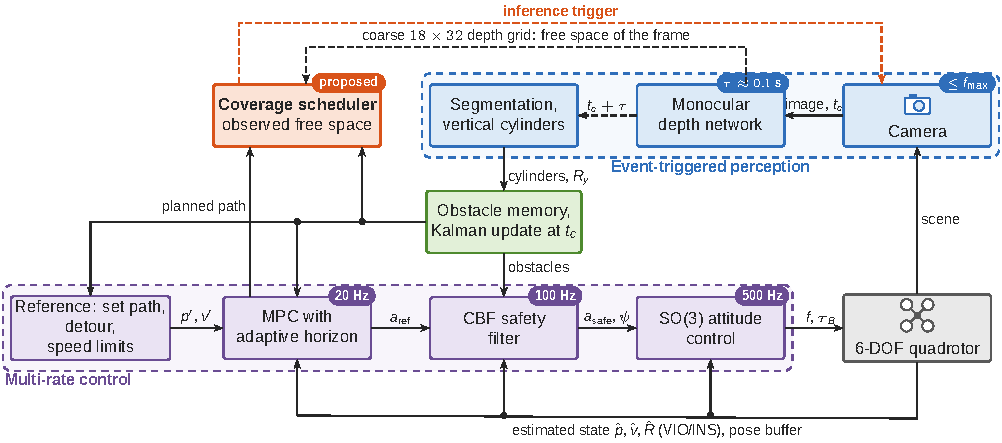
\includegraphics[width=\textwidth]{Fig1.pdf}
\caption{Multi-rate closed-loop architecture. The perception branch (upper dashed frame) is event-triggered: the
coverage scheduler (bold block, the contribution of this paper) triggers a capture when the planned path leaves the
observed free space, at a rate not exceeding $\fmax$; the depth network result arrives after the latency $\tau$ and
enters the obstacle memory through a Kalman update at the capture time $t_c$. The control branch (lower dashed frame)
is periodic; the tag on each block gives its rate or latency. Dashed arrows: asynchronous signals}
\label{fig:arch}
\end{figure}

\subsection{Vertical cylinders and delay-compensated memory}\label{sec:memory}

\runin{Segmentation.} The depth image is split into connected regions according to the log-depth difference between
neighbouring pixels; outliers, edge pixels (large log-depth gradient) and pixels mixed between two surfaces are
removed; regions smaller than 12 pixels are discarded.

\runin{Cylinders.} The vertical direction is taken from the attitude at the capture time (on hardware: the gravity
direction of the inertial measurement unit). For each region, let $u_p$ be the horizontal direction and $r_p$ the
horizontal range of pixel $p$, $\bar u$ the normalized mean direction, $\varphi_p = \angle(u_p,\bar u)$ and
$\alpha = \max_p\varphi_p + \delta/2$, with $\delta$ the angle subtended by one pixel. A vertical cylinder of radius
$\rho$ whose axis lies at distance $D$ from the camera in direction $\bar u$ is seen under the half-angle $\alpha$ with
$\sin\alpha = \rho/D$, and the ray at $\varphi_p$ hits its front surface at
$r_p = D\,(\cos\varphi_p - \sqrt{\sin^2\alpha - \sin^2\varphi_p})$. Each pixel therefore yields an estimate of $D$,
and
\begin{equation}\label{eq:cyl}
\begin{aligned}
\hat D &= \operatorname*{median}_{\varphi_p \le 0.8\alpha}
\frac{r_p}{\cos\varphi_p - \sqrt{\sin^2\alpha - \sin^2\varphi_p}},\\
\rho &= \max\!\Big(\hat D\sin\alpha,\; q_{0.9}\big(\|P_h x_p - \hat D\bar u\|\big)
- z_{0.9}\,\sigma_{\mathrm{px}}(\hat D)\,\hat D\Big),
\end{aligned}
\end{equation}
where $P_h$ is the projection onto the horizontal plane, $q_{0.9}$ is the 90\,\% quantile, and the second term covers
90\,\% of the points of the region (minus the expected spread of the pixel noise) for shapes other than circular
cylinders. Regions whose horizontal half-width exceeds $2~\text{m} + 0.1\times$ the distance are split in two along
the principal axis, recursively, so that a wall becomes a row of cylinders. The bottom and top are the lowest and
highest observed points. If a region touches the upper or lower image border, or the pixel directly below (above) it
is closer to the camera, the corresponding end is considered unobserved and the cylinder is extended to the ground
(upwards) until that end is observed. Low objects such as vehicles and high tree crowns therefore do not block the
flight altitude, as they would when enclosed by spheres. The measurement covariance $R_y$ includes contributions from
the scale error, the shift, the correlated error field, the far-range bias, the pixel noise and the angular
quantization.

\runin{Delay-compensated memory.} Each cylinder is a static landmark with axis position $c$, covariance $P$, radius
$\rho$, bottom and top. The measurement $y = \hat p(t_c) + \hat R(t_c)\,(p_{BC} + R_{BC}\,c_C)$ is formed with the
estimated pose at the capture time, taken from a pose buffer; the Kalman update is applied at $t_c$ to the value
predicted from the latest posterior and then predicted to the current time. Following the definition
in~\cite{barshalom2002}, a measurement is out of sequence only if the track has already been updated to a time later
than its time stamp; the single-frame-in-process assumption excludes this case, so measurements are processed in time
order, and in the example of~\cite{barshalom2002} processing in time order gives the same result as the optimal
processor. The exact solution of~\cite{barshalom2002} assumes a linear--Gaussian system, correct data association and
a delay within one sampling period. In our system, association without identities, a scale error shared by all objects
of a frame and the pose error at $t_c$ fall outside these assumptions, so the update is approximate. A detection $k$
is associated with track $i$ only if the Mahalanobis distance satisfies
$e_{ik} = \nu_{ik}^\top S_{ik}^{-1}\nu_{ik} \le 16.27$ ($\chi^2_3$, 99.9\,\%), and assignment is greedy nearest
neighbour with cost $e_{ik} + \ln\det S_{ik}$. The radius is smoothed with factor 0.3; an unobserved end is replaced
by the measured value the first time it is observed. Unassociated detections that lie inside an existing cylinder
are ignored; the remaining ones create new tracks. A track is deleted when (a) it is predicted to be in the image and
not occluded but is not associated in 3 consecutive frames, or (b) it is outside the field of view and more than
10~m from the UAV. Between frames, the covariance grows with the process noise.

\runin{Locally equivalent sphere.} Blocks that use first-order conditions at the UAV position $p$ (CBF filter, risk
quantities, scheduler, speed limits) replace each cylinder by a sphere of the same radius centred at
$c_{\mathrm{eff}} = q - \rho\,n$, where $q$ is the point of the cylinder surface closest to $p$ and $n$ is the outward
normal at $q$; then $\|p - c_{\mathrm{eff}}\| - \rho$ equals the distance to the cylinder and the two gradients
coincide. The MPC linearizes the cylinders at each predicted point in the same way.

\subsection{Scheduling by observed free space}\label{sec:scheduler}

\runin{Free space of one frame.} The coarse depth grid $G_k$ of frame $k$ divides the image into $18\times32$ cells;
each cell holds the 20\,\% quantile of the valid depths in the cell, or $\infty$ if fewer than 20\,\% of its pixels
are valid. The grid is capped at $\Reff$ and then minimized over a $3\times3$ neighbourhood,
$\tilde G_k = \min_{3\times3}\min(G_k,\Reff)$, so that a tube around the path, not only its centre line, has to be
free. Let $z_k(x)$ be the depth of point $x$ in the optical frame of frame $k$ (with the pose at the capture time) and
$\kappa_k(x)$ the cell into which $x$ projects. The free space observed by frame $k$ is
\begin{equation}\label{eq:free}
\Fs_k = \big\{x:\ z_k(x) > 0.3~\text{m},\ \kappa_k(x)\ \text{not on the grid border},\
z_k(x) + d_s \le \tilde G_k(\kappa_k(x))\big\},
\end{equation}
i.e.\ the points lying at least $d_s$ in front of the measured surface; space behind a surface (occluded), outside the
field of view or beyond $\Reff$ does not belong to $\Fs_k$. The observed free space at time $t$ is the union over the
$K = 8$ most recent frames with results, $\Fs(t) = \bigcup_{k\in\mathcal K(t)}\Fs_k$.

\runin{Coverage condition.} Let $\sigma_t(s)$ be the planned path of the MPC parametrized by arc length $s$, with
$\sigma_t(0) = p(t)$, extended straight along its final direction if it is shorter than needed, and let
$v = \|v(t)\|$. The distance that has to be observed is
\begin{equation}\label{eq:need}
\ell(v) = v\,\tauh + \frac{v^2}{2a_b} + d_s,
\end{equation}
i.e.\ the distance flown while waiting for the result of a frame captured now, plus the braking distance and a margin
$d_s = 0.5$~m. The coverage condition is
\begin{equation}\label{eq:cov}
C(t):\qquad \sigma_t(s) \in \Fs(t)\quad \forall s \in [s_0,\ \ell(v)],
\end{equation}
with $s_0 = 1$~m (closer points lie within the safety margin). The conservative latency estimate is
$\tauh = \mu_\tau + 2\sigma_\tau$, where $\mu_\tau$ and $\sigma_\tau$ are updated by exponential moving averages
(factor 0.2) from the measured latency of each result.

\runin{Trigger rule.} At every control step (100~Hz), a frame is captured when
\begin{equation}\label{eq:trig}
\begin{aligned}
\mathrm{trig}(t) &= I(t) \wedge \big[\neg C(t) \vee e_\sigma(t) \vee e_{\mathrm{em}}(t) \vee
(v < v_{\mathrm{stall}})\big],\\
I(t) &= (\text{no frame in process}) \wedge (t - t_{\mathrm{last}} \ge 1/\fmax).
\end{aligned}
\end{equation}
The uncertainty event $e_\sigma$ occurs when an object that can be re-observed is close (conservative distance below
8~m), has a position standard deviation of at least 0.6~m and a variance larger than twice that of a new measurement
at that distance (information-gain filtering): an object first seen from far away keeps a large covariance, and
cylinders inflated by uncertainty can close narrow gaps until they are measured again from close range. The emergency
event $e_{\mathrm{em}}$ occurs when an object on a collision course has a stopping margin
$d^c - d_s - v_c^2/(2a_b) \le 0$, with $d^c$ the conservative distance and $v_c$ the approach speed. When the UAV is
nearly stationary ($v < v_{\mathrm{stall}} = 1$~m/s), frames are captured continuously at $\fmax$ to re-measure the
surrounding objects from close range. Known objects do not trigger frames by themselves, since they are already in the
memory. The cap $\fmax$ applies to all events, including emergencies: in event-triggered safety-critical control, the
error dynamics need not vanish when the quantity that decides the triggering vanishes, so control updates may
accumulate~\cite{taylor2020}; the hard cap is a design lower bound on the interval between two captures.

\runin{Property of the coverage condition.} The following proposition states what condition~\eqref{eq:cov}
guarantees.

\begin{assumption}\label{as:cov}
(A1) Obstacles are static. (A2) Every point of $\Fs(t)$ is at least $r_b$, the collision radius of the UAV, away from
obstacle surfaces. (A3) During $[t, t+\tauh]$, the UAV moves along $\sigma_t$ with a speed not exceeding
$v = \|v(t)\|$, and it can decelerate along $\sigma_t$ at $a_b$ from any instant. (A4) The segment $\sigma_t([0,s_0])$
is collision-free.
\end{assumption}

\begin{proposition}\label{prop:cov}
Suppose that Assumption~\ref{as:cov} holds and that $C(t)$ is satisfied. For every $t_b \in [t, t+\tauh]$, the
manoeuvre ``follow $\sigma_t$ until $t_b$, then brake at $a_b$'' brings the UAV to rest at $\sigma_t(s^*)$ with
$s^* \le \ell(v) - d_s$, the whole segment $\sigma_t([0,s^*])$ is collision-free, and the part of the path ahead of the
stopping point up to $\ell(v)$ lies in observed free space.
\end{proposition}

\begin{proof}
By (A3), the distance flown during $[t, t_b]$ does not exceed $v(t_b - t) \le v\tauh$ and the speed at $t_b$ does not
exceed $v$, so the braking distance does not exceed $v^2/(2a_b)$. Hence $s^* \le v\tauh + v^2/(2a_b) = \ell(v) - d_s$.
For $s\in[s_0, \ell(v)]$, $C(t)$ gives $\sigma_t(s)\in\Fs(t)$; by (A2) these points are at least $r_b$ away from
obstacles at the time of observation, and by (A1) this remains true at every later time. For $s\in[0,s_0]$, the
statement follows from (A4).
\end{proof}

A frame captured at any time in $[t, t+\tauh]$ returns its result only after $\tau \le \tauh$, so no new information
can change the ability of the UAV to stop before $t + \tauh$. Proposition~\ref{prop:cov} states that when $C(t)$
holds, the ability to stop within observed space persists throughout that interval without a new frame; skipping the
inference at $t$ therefore loses nothing in terms of stopping ability. When $C(t)$ does not hold, the available data
are insufficient to certify such a stopping manoeuvre, and only a new frame can extend $\Fs$; rule~\eqref{eq:trig}
captures as soon as the cap allows.

\begin{corollary}\label{cor:rate}
Ignoring older frames and other events, if the most recent frame observes free space along the path up to a depth $D$
from the capture position and the UAV flies at a nearly constant speed $v$, then condition~\eqref{eq:cov} based on
that frame holds until the UAV has travelled $D - \ell(v)$ since the capture. The interval between two captures
triggered by coverage is therefore approximately $(D - \ell(v))/v$, bounded below by $1/\fmax$, and it decreases when
$D$ decreases (dense obstacles, occlusion, detours) or when $v$ increases.
\end{corollary}

\begin{remark}[Rate cap and speed limit]\label{rem:cap}
When $C(t)$ does not hold but $I(t)$ is false (a frame is in process, or less than $1/\fmax$ has elapsed since the
previous capture), the needed frame is delayed and Proposition~\ref{prop:cov} no longer applies. The speed
limit~\eqref{eq:vperc} of Section~\ref{sec:speed} compensates for this delay in open space: if the free space of the
latest frame along the path extends to $\Reff$, the next result arrives no later than $T_r$ after that capture,
and~\eqref{eq:vperc} ensures that the UAV can still stop within the free space of that frame. When obstacles or
occlusion make the free space shorter than $\Reff$, the cap can delay the needed frame, and safety relies on the
memory and the CBF filter. Testable prediction: the collision rate rises sharply when $1/\fmax$ becomes comparable to
the time the UAV needs to consume the short free space in dense regions (Section~\ref{sec:r1}).
\end{remark}

\begin{remark}[Discretization and acceleration]
Condition~\eqref{eq:cov} is evaluated at 100~Hz with the current speed; the extra distance flown in one step,
$v\Delta t_c \le 0.15$~m, is smaller than $d_s$, so the stopping point still lies in the checked segment. If the UAV
accelerates during $[t, t+\tauh]$, (A3) is violated; re-evaluation at every step increases $\ell(v)$ accordingly and
makes $C$ fail earlier, but~\eqref{eq:need} contains no acceleration term.
\end{remark}

\begin{remark}[Scope]\label{rem:scope}
Proposition~\ref{prop:cov} concerns the scheduling decision, not the safety of the closed loop: the MPC and the CBF
filter constrain the motion with respect to the objects in the memory, not with respect to $\Fs$; (A2) can be violated
by depth errors; and the track deletion rules can remove an observed object from the memory. Closed-loop safety is
therefore evaluated empirically.
\end{remark}

\begin{figure}[t]
\centering
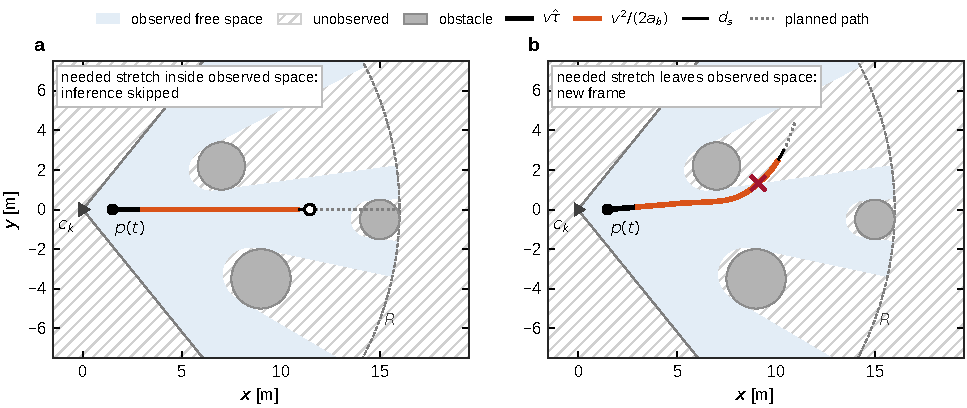
\includegraphics[width=\textwidth]{Fig2.pdf}
\caption{Coverage condition~\eqref{eq:cov}, sketched in the horizontal plane for one frame captured at $c_k$
($102^\circ$ field of view; $R$ stands for $\Reff$). The observed free space extends to the measured surface minus
$d_s$; space behind objects, outside the field of view or beyond $R$ is unobserved (hatched). The UAV at $p(t)$ with
$v = 10$~m/s must have observed the path stretch made of $v\tauh$ (waiting for the result), $v^2/(2a_b)$ (braking) and
$d_s$. \textbf{a} Straight path: the whole stretch lies in observed space and the inference is skipped. \textbf{b}
Detour behind an object: the stretch enters occluded space (cross) and a new frame is triggered}
\label{fig:cov}
\end{figure}

\subsection{Speed limits}\label{sec:speed}

The reference speed is the minimum of three limits. Besides the physical limit $v_{\max}$, the perception-range limit
requires that an object appearing at the boundary $\Reff$ can still be avoided by braking after the worst-case
reaction time:
\begin{equation}\label{eq:vperc}
v\,T_r + \frac{v^2}{2a_b} + d_s \le \Reff,\qquad T_r = \max(1/\fmax,\ \tauh) + \tauh,
\end{equation}
which has the form of the condition of~\cite{liu2016} with the additional margin $d_s$; $T_r$ consists of the waiting
time until the next capture (bounded by the cap and by the frame in process) plus the latency. With
$\tauh \approx 0.14$~s, this limit is 8.9, 12.1 and 13.5~m/s at $\fmax = 0.5$, 1 and 1.5~Hz, and exceeds $v_{\max}$
from $\fmax = 3$~Hz. The obstacle-density limit requires the approach speed to every object $i$ in the flight corridor
ahead to allow braking,
\begin{equation}\label{eq:vclut}
v\cos\theta_i \le k_c\sqrt{2a_b\max(d^c_i - d_s,\,0)},\qquad k_c = 0.9,
\end{equation}
where $\theta_i$ is the angle between the flight direction and the direction to the object, and is not lower than
1.5~m/s. These limits use a point-mass model and consider only braking: lateral evasion takes less time than braking
at high speed~\cite{falanga2019}, so the stopping distance used here is conservative, whereas the point-mass model
neglects the rotational dynamics~\cite{loquercio2021}.

\subsection{Reference, MPC and CBF filter}\label{sec:control}

\runin{Reference.} The UAV tracks the set path. When a stretch ahead is blocked by a cylinder in the memory (including
the margin), the reference switches to the shortest collision-free path (a polygon around the cylinders at flight
altitude) to a rejoin point after the blocked stretch, and the deviation from the set path is not penalized
meanwhile. Objects lower than the flight altitude can be overflown.

\runin{MPC.} The MPC uses a double-integrator model with step $\Delta t = 0.1$~s and a horizon of $N\in[10,30]$ steps,
chosen from the time to collision, the braking distance and the expected arrival time of the next perception result.
The problem is
\begin{equation}\label{eq:mpc}
\min_{u,\ s\ge0}\ \sum_{j=1}^{N}\Big(\|p_j - p_j^r\|^2_{Q_p} + \|v_j - v_j^r\|^2_{Q_v} + \|u_{j-1}\|^2_{R}
+ \|u_{j-1} - u_{j-2}\|^2_{S}\Big) + \sum_i\big(w_1 s_i + w_2 s_i^2\big)
\end{equation}
subject to box constraints on acceleration, velocity and altitude and, for each object $i$ among the 8 nearest,
\begin{subequations}\label{eq:mpccon}
\begin{align}
g_{ij}(p_j) &\ge -s_i, && j = 1,\dots,N, \label{eq:mpca}\\
g_{ij}(p_j) &\ge (1-\gamma)\,g_{ij}(p_{j-1}) - s_i, && j = 1,\dots,N_d, \label{eq:mpcb}\\
\|v_N\|_\infty &\le \varepsilon_v, \label{eq:mpcc}
\end{align}
\end{subequations}
where $g_{ij}(p) = n_{ij}^\top(p - c_{ij}) - d_{ij}$, $c_{ij}$ is the centre of the equivalent sphere of the cylinder
at the linearization point of step $j$ (from the previous solution), $n_{ij}$ is the unit normal of the tangent
half-space (horizontal unless the object is entirely above or below, and rotated sideways when nearly head-on), and
$d_{ij} = \rho_i + d_s + \beta\sigma_{ij}$ is the inflated radius, with $\sigma_{ij}$ the predicted position standard
deviation at step $j$; $\beta = 2$ is an empirical factor, not tied to a probability level.
Constraint~\eqref{eq:mpca} is sufficient for $\|p_j - c_{ij}\| \ge d_{ij}$ for any unit normal and keeps the problem a
QP; \eqref{eq:mpcb} is a discrete-time CBF row~\cite{zeng2021} on the same plane for the first $N_d = 10$ steps;
\eqref{eq:mpcc} requires the plan to end at rest, which corresponds to the committed stopping trajectory
of~\cite{liu2016}. In $\sigma_{ij}$, the covariance is reduced at the steps where a perception result is expected if
the object lies in the expected field of view; the mean is not updated. Inflating by the covariance along the horizon
is similar to~\cite{zhu2019}. When the problem is infeasible, a braking command is used instead. The QP is solved by a
Mehrotra-type primal--dual predictor--corrector interior-point method~\cite{mehrotra1992}, written in plain MATLAB.

\runin{CBF filter.} For each object within the range of action, let $r = c_{\mathrm{eff}} - p$, the clearance
$s = \|r\| - d$ with $d = \rho + d_s + \beta\sigma$, and the approach speed $v_c = \hat r^\top v$. The braking
barrier~\cite{wang2017}
\begin{equation}\label{eq:hbrake}
h = \sqrt{2a_b\,s} - v_c
\end{equation}
is positive if and only if $v_c^2 < 2a_b s$, i.e.\ the UAV can stop before the inflated surface when braking at
$a_b$ --- the same braking condition as the emergency event and the limit~\eqref{eq:vclut}. The condition
$\dot h \ge -\alpha h$ gives a linear constraint on the commanded acceleration $a$:
\begin{equation}\label{eq:cbfrow}
\hat r^\top a \le \alpha h - \frac{a_b\,(v_c + \dot d)}{\sqrt{2a_b s}} + \frac{\|v_\perp\|^2}{\|r\|} - \delta_a,
\end{equation}
where $v_\perp$ is the velocity component orthogonal to $\hat r$ and $\dot d$ is the growth rate of the inflated
radius due to the growing covariance. The filter solves $\min\|a - a_{\mathrm{ref}}\|^2 + w\,\epsilon^2$ subject to
rows~\eqref{eq:cbfrow}, two altitude rows and ``blind-motion'' rows that keep the speed opposite to the camera viewing
direction below 1.5~m/s and the speed out of the field-of-view edges below 1~m/s, similar to the constraint that keeps
the velocity within the sensor's field of view in~\cite{misyats2025}. The slack $\epsilon$ is nonzero only when the
rows are incompatible; the solution is then the least-violating one~\cite{yaghoubi2021}, and $h \ge 0$ is no longer
guaranteed. The safe acceleration and the yaw angle are converted into the total thrust and the desired attitude of
the geometric tracking controller of~\cite{lee2010}, used in simplified form (zero desired angular velocity, so that its
feed-forward terms vanish; per-axis gains; tilt and thrust limits; drag compensation) at 500~Hz; the stability results
of~\cite{lee2010} are not claimed for this simplified form.

\subsection{Baselines}\label{sec:baselines}

\textbf{FR} (fixed rate) captures uniformly at exactly $\fmax$. \textbf{RA} (risk-adaptive) chooses the capture
interval from the open-loop safe time: for each visible object, the longest time for which the UAV, with its current
approach speed, could still stop without a new image, accounting for the growing covariance, together with a
hypothetical object at the boundary of the trusted range along the flight direction; the interval is the minimum of
these times minus $\tauh$, with distance, uncertainty and emergency events. RA resembles the safe time window of
self-triggered control~\cite{yang2019} and the derivation of a minimum rate from the tolerable
latency~\cite{hsiao2022}. \textbf{COV-NC} is COV without the limit~\eqref{eq:vclut}. All variants use the same
memory, MPC, CBF filter, limit~\eqref{eq:vperc} and cap $\fmax$. Table~\ref{tab:params} lists the main parameters.

\begin{table}[t]
\caption{Main parameters (all variants)}\label{tab:params}
\begin{tabular}{@{}lp{4.6cm}p{4.4cm}@{}}
\toprule
Block & Parameter & Value \\
\midrule
Quadrotor & mass; $T/W$; collision radius $r_b$ & 1~kg; 2.4; 0.25~m \\
 & $\theta_{\max}$; $a_b$; $v_{\max}$ & $46^\circ$; 6.2~m/s$^2$; 15~m/s \\
Camera, network & field of view; network input; $\Reff$ & $102^\circ\times70^\circ$; $320\times180$; 26~m \\
 & latency (capture + transfer + inference) & $10 + 10 + 80$~ms (log-normal, CV 0.25) \\
Scheduler & $\fmax$ (default); $K$; grid & 0.5--5~Hz (3~Hz); 8 frames; $18\times32$, 20\,\% quantile \\
 & $d_s$; $s_0$; $v_{\mathrm{stall}}$; $\tauh$ & 0.5~m; 1~m; 1~m/s; $\mu_\tau + 2\sigma_\tau$ \\
Memory & $\chi^2_3$ gate; deletion after; forgetting outside view & 16.27; 3 frames; 10~m \\
MPC & rate; $\Delta t$; $N$; $N_d$; $\gamma$; $\beta$ & 20~Hz; 0.1~s; 10--30; 10; 0.3; 2 \\
CBF & rate; $\alpha$; $\delta_a$ & 100~Hz; 3~s$^{-1}$; 0.3~m/s$^2$ \\
Attitude & rate; model integration & 500~Hz; RK4, 2~ms \\
\botrule
\end{tabular}
\end{table}

% =====================================================================================================================
\section{Experimental setup}\label{sec:setup}

\runin{Scenarios.} Table~\ref{tab:grid} summarizes the three scenario families. SN (nominal flight) consists of 300~m
routes with 1--3 segments at 2--3.5~m altitude, divided into zones of 40--80~m: 35\,\% empty, 40\,\% sparse (1--3
objects), 25\,\% dense (6--12 objects), with gaps of at least 3.5~m. In SH (hard), all zones are dense, haze
(visibility 200~m) is present in the worlds with odd index, and two vehicles cross the route (2--4~m/s) in the worlds
whose index is divisible by 3; the vehicles are not announced to the algorithm, and collisions with them are counted
separately because they fall outside the static-obstacle assumption. SE (everyday scenes) consists of straight 200~m
routes in six scene types with 5 worlds each: open field, a single tree on the route, an avenue lined with trees on
both sides, cars parked along the road and a truck on the route, buildings along the route, and a street canyon.

\runin{Test grid.} Each variant runs on the same worlds, the same three commanded speeds (6, 10, 15~m/s) and the same
ten caps $\fmax$ (0.5--5~Hz in steps of 0.5~Hz), so all comparisons are paired. The main part uses the default camera
with COV, FR, RA and COV-NC (14\,400 runs); the camera part runs COV and FR with three other cameras (21\,600 runs);
36\,000 runs in total.

\runin{Outcomes and metrics.} A run ends at the goal, at a collision (body-to-object distance equal to zero) or when
stuck (less than 1~m of progress along the set path in 60~s); the flight time is not limited. The metrics are the
collision rate with static objects, the rate of stuck runs, the number of inferences per mission, the actual frame rate
and the time to goal. Rates are compared with two-sided Fisher exact tests on run counts. When variants are compared,
the caps 1.5--5~Hz are pooled, because Section~\ref{sec:r1} shows that this is the range in which the collision rate
no longer depends on the cap. No correction for multiple testing is applied, so $p$ values close to 0.05 are
interpreted with caution.

\runin{Implementation.} All algorithms are written in MATLAB, and the Simulink model is generated from the same code.
The test grid is run with a MATLAB simulation engine that uses the same functions and the same multi-rate structure as
the Simulink model, on GitHub Actions; the quadrotor model is integrated by fourth-order Runge--Kutta with a 2~ms step.
The source code, the per-run results and the scripts that produce the tables and figures are publicly available at
\url{https://github.com/nxbnxb1/project1} (see Statements and Declarations).

\runin{Use of AI tools.} Parts of the simulation code, the analysis scripts and
the first draft of this manuscript were prepared with the assistance of an AI coding assistant based on a large
language model (Claude, Anthropic). The author specified the method and the experiments, reviewed and tested the
code, checked the reported numbers against the stored simulation logs and the cited statements against the full texts
of the cited works, and takes full responsibility for the content.

\begin{table}[t]
\caption{Scenarios and test grid}\label{tab:grid}
\renewcommand{\thefootnote}{\alph{footnote}}% table notes: lower-case letters
\begin{tabular}{@{}llcl@{}}
\toprule
Scenario & Characteristics & Worlds & Runs (default camera) \\
\midrule
SN & 300~m route; empty / sparse / dense zones & 60 & 7\,200 \\
SH & all zones dense; haze; crossing vehicles\footnotemark[1] & 30 & 3\,600 \\
SE & 200~m route; six everyday scene types & 30 & 3\,600 \\
\midrule
\multicolumn{4}{@{}l}{Each world: 3 commanded speeds $\times$ 10 caps $\fmax$ $\times$ 4 variants (COV, FR, RA,
COV-NC)} \\
\multicolumn{4}{@{}l}{Camera part: 3 other cameras $\times$ 2 variants (COV, FR) on the same grid: 21\,600 runs} \\
\botrule
\end{tabular}
\footnotetext[1]{Collisions with vehicles are outside the scope (static-obstacle assumption) and are counted separately.}
\end{table}

% =====================================================================================================================
\section{Results}\label{sec:results}

Each subsection below tests one claim: it states the prediction derived from Section~\ref{sec:method}, the test, and
the conclusion.

\subsection{Mechanism in one mission}\label{sec:r0}

Figure~\ref{fig:mission} compares COV and FR in the same SN world with $v_{\mathrm{des}} = 10$~m/s and
$\fmax = 3$~Hz. FR captures uniformly at $\fmax t$ (108 inferences). COV concentrates its inferences on the stretches
with obstacles and on detours, almost stops capturing on the open stretch from about 12~s to 19~s and while slowing
down near the goal (64 inferences). The two variants keep minimum clearances of 1.7~m and 0.7~m, both larger than
$d_s - r_b$, and reach the goal after 33.7~s and 36.4~s. This mission illustrates the mechanism of the thesis: the
number of frames needed is determined by the amount of unobserved space that the path consumes, not by the flight
time.

\begin{figure}[t]
\centering
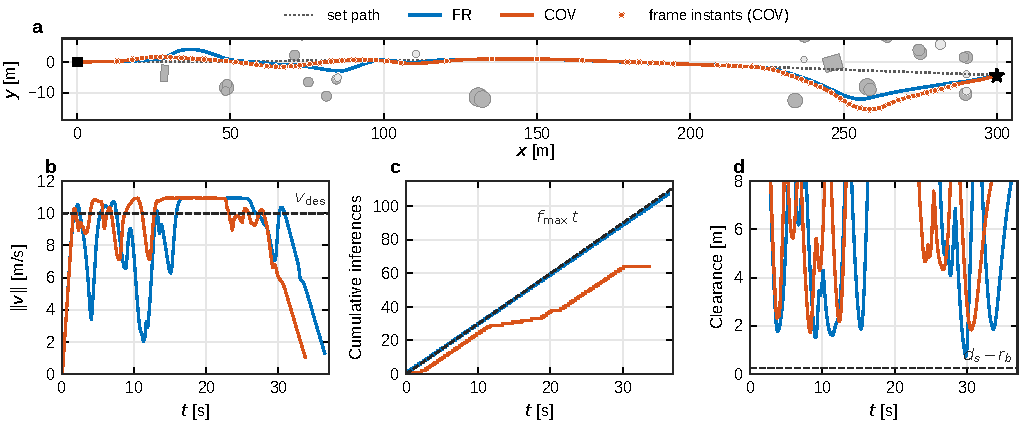
\includegraphics[width=\textwidth]{Fig3.pdf}
\caption{One SN mission (world 22, $v_{\mathrm{des}} = 10$~m/s, $\fmax = 3$~Hz) with COV and FR. \textbf{a} Path,
obstacles (dark fill: objects that intersect the flight altitude) and the capture instants of COV. \textbf{b} Speed.
\textbf{c} Cumulative number of inferences; dashed: $\fmax t$. \textbf{d} Distance from the UAV body to the nearest
obstacle; dashed: $d_s - r_b$}
\label{fig:mission}
\end{figure}

\subsection{Claim 1: safety requires a minimum rate and saturates above it}\label{sec:r1}

\runin{Prediction.} If the remaining collisions were due to a lack of new information, the collision rate would have to
decrease as the cap increases. By Remark~\ref{rem:cap}, this should hold only at low caps, where the cap delays the
needed frame in dense regions.

\runin{Result.} Figure~\ref{fig:rate}a confirms the prediction. Pooling the four schedulers, the collision rate in SN
drops from 27\,\% at 0.5~Hz to 6.7\,\% at 1~Hz and 3.8\,\% at 1.5~Hz (1~Hz versus 1.5~Hz: $p = 0.009$). From 2~Hz to
5~Hz there is no statistically significant difference (SN 3.2\,\% and 2.4\,\%, $p = 0.34$; SH 8.3\,\% and 8.3\,\%,
$p = 1$; SE 0.6\,\% and 0.8\,\%, $p = 0.69$). Figure~\ref{fig:rate}b shows that COV is limited by the cap at 0.5~Hz
(0.44--0.49 frames/s) and close to it at 1~Hz (0.73--0.89 frames/s); from 1.5~Hz on, the actual rate departs
increasingly from the cap and is only 2.3--3.0 frames/s at 5~Hz. The rate cap was respected in all 36\,000 runs: the
smallest interval between two captures was not shorter than $1/\fmax$ by more than one 10~ms control step. At caps from
1.5~Hz, the rate of stuck runs is 0--0.4\,\% for all variants, except COV-NC in SH (1.2\,\%).

\runin{Conclusion.} Above about 2~Hz, the remaining collisions are not due to the perception rate. When the cap is
high enough not to bind, COV selects a rate well below the cap.

\begin{figure}[t]
\centering
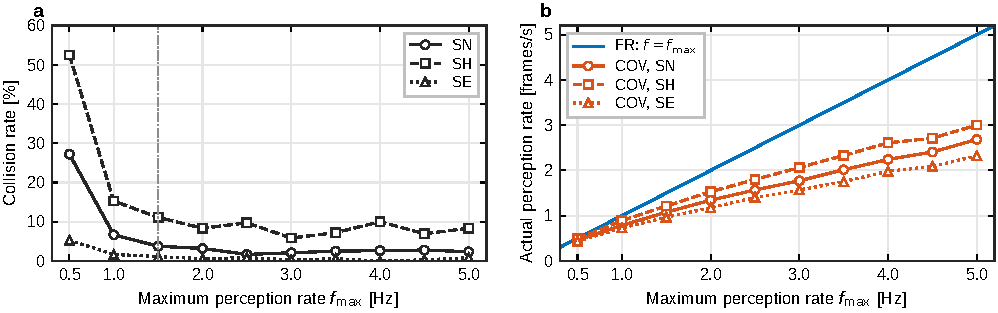
\includegraphics[width=\textwidth]{Fig4.pdf}
\caption{Effect of the rate cap (default camera). \textbf{a} Collision rate with static objects, pooled over the four
schedulers (720 runs per point in SN, 360 in SH and SE); vertical line: 1.5~Hz. \textbf{b} Actual frame rate of COV
compared with FR, which captures at exactly $\fmax$}
\label{fig:rate}
\end{figure}

\subsection{Claim 2: fewer inferences at the same safety level}\label{sec:r2}

\runin{Prediction.} By Proposition~\ref{prop:cov}, at the instants at which the coverage condition holds, a new frame
does not increase the ability to stop; FR still captures at those instants. With the same memory and the same safety
layers, COV should therefore reach a collision rate equivalent to that of FR at the same cap with fewer inferences.

\runin{Result.} Table~\ref{tab:compare} confirms the prediction in SN and SE. Pooling the caps 1.5--5~Hz, the static
collision rates of COV and FR are 2.4\,\% and 2.0\,\% in SN ($p = 0.53$) and 0.3\,\% and 0.4\,\% in SE ($p = 1$),
while COV uses 0.54--0.72 (SN) and 0.50--0.63 (SE) times the inferences of FR at the same cap, computed over the runs
in which both reach the goal. This ratio decreases as the cap increases, because FR captures at the cap whereas COV
captures on demand (Fig.~\ref{fig:rate}b). In SH, COV uses 0.61--0.81 times the inferences and has a collision rate of
8.2\,\% versus 5.8\,\% ($p = 0.098$): the difference is not significant at the 0.05 level, but equivalence cannot be
concluded. In continuously dense scenes the free space ahead is always short, so the fraction of time in which COV
skips inferences, and the savings, are smaller.

A comparison at the same cap does not answer a more practical question: given a computational budget, how should it
be spent? Pairing COV at cap $2f$ with FR at cap $f$ ($f = 1$, 1.5, 2, 2.5~Hz) gives approximately equal numbers of
inferences per mission (in SN, COV uses 0.99--1.19 times as many as FR). In SN, the total number of failed runs
(static collisions and stuck runs) is 16 versus 35 of 720 ($p = 0.0096$); the difference is concentrated in the
2~Hz--1~Hz pair, where FR lies in the non-saturated rate range. In SH (31 and 43 of 360, $p = 0.18$, with COV using
7--24\,\% more inferences) and SE (0 and 5 of 360, $p = 0.062$), the differences are not statistically significant.

The obstacle-density limit~\eqref{eq:vclut} makes no significant difference in safety: COV-NC has collision rates of
2.2\,\%, 7.5\,\% and 0.4\,\% versus 2.4\,\%, 8.2\,\% and 0.3\,\% for COV ($p \ge 0.7$), a rate of stuck runs in SH of
1.2\,\% versus 0.3\,\% ($p = 0.064$), and a shorter time to goal (SN, 15~m/s: 33.5~s versus 36.4~s). In this grid,
the CBF filter with the same braking condition and limit~\eqref{eq:vperc} suffices to maintain the safety level;
block~\eqref{eq:vclut} mainly slows the reference down before the filter has to intervene.

\runin{Conclusion.} At the same cap, the coverage condition removes 28--50\,\% of the inferences in SN and SE without a
statistically significant difference in safety; at the same budget, setting a high cap and letting the coverage
condition decide when to capture is not worse, and at a low budget better, than capturing uniformly at the rate that
the budget allows.

\begin{table}[t]
\caption{Comparison of the schedulers with the default camera, pooled over $\fmax = 1.5$--5~Hz (SN 1\,440 runs per
variant; SH and SE 720)}\label{tab:compare}
\renewcommand{\thefootnote}{\alph{footnote}}% table notes: lower-case letters
\begin{tabular}{@{}llcccc@{}}
\toprule
Scenario & Scheduler & Static collisions [\%] & $p$ vs.\ COV\footnotemark[1] & Stuck [\%] & Frames/s\footnotemark[2] \\
\midrule
\multirow{4}{*}{SN} & COV (proposed) & 2.4 & --- & 0.2 & 1.89 \\
 & FR & 2.0 & 0.53 & 0.3 & 3.23 \\
 & RA & 3.9 & 0.033 & 0.3 & 1.89 \\
 & COV-NC & 2.2 & 0.71 & 0.1 & 1.87 \\
\midrule
\multirow{4}{*}{SH} & COV (proposed) & 8.2 & --- & 0.3 & 2.16 \\
 & FR & 5.8 & 0.098 & 0.4 & 3.22 \\
 & RA & 12.2 & 0.015 & 0.4 & 2.28 \\
 & COV-NC & 7.5 & 0.70 & 1.2 & 2.16 \\
\midrule
\multirow{4}{*}{SE} & COV (proposed) & 0.3 & --- & 0.0 & 1.66 \\
 & FR & 0.4 & 1 & 0.0 & 3.23 \\
 & RA & 1.1 & 0.11 & 0.1 & 1.87 \\
 & COV-NC & 0.4 & 1 & 0.0 & 1.64 \\
\botrule
\end{tabular}
\footnotetext[1]{Two-sided Fisher exact test on the counts of static collisions.}
\footnotetext[2]{Mean frame rate; FR captures at exactly $\fmax$, so its value is close to the mean of the caps (3.25~Hz).}
\end{table}

\subsection{Claim 3: the frame rate adapts to obstacle density}\label{sec:r3}

\runin{Prediction.} By Corollary~\ref{cor:rate}, the interval between two captures of COV decreases when the depth of
the free space ahead decreases, i.e.\ when obstacles become denser.

\runin{Result.} Figure~\ref{fig:dens} divides the flight time in SN ($v_{\mathrm{des}} = 15$~m/s, $\fmax = 3$~Hz)
according to the number of objects within a radius of 15~m. The frame rate of COV increases from 1.76~frames/s with no
object to 2.59~frames/s with 6 or more objects, whereas FR keeps 2.94--2.99~frames/s regardless of density. At the
same time, the mean speed of COV decreases from 11.2 to 3.8~m/s because of the limits~\eqref{eq:vperc}--\eqref{eq:vclut}
and the detours. By Corollary~\ref{cor:rate}, a lower speed by itself lengthens the interval between captures; the
frame rate nevertheless increases, so the increase comes from the shorter free space and from the uncertainty and
emergency events, which occur only near obstacles, and not from the speed.

\runin{Conclusion.} The same trigger rule yields a low rate in open space and approaches the cap in dense regions ---
which a fixed rate achieves only if it is set for the dense regions.

\begin{figure}[t]
\centering
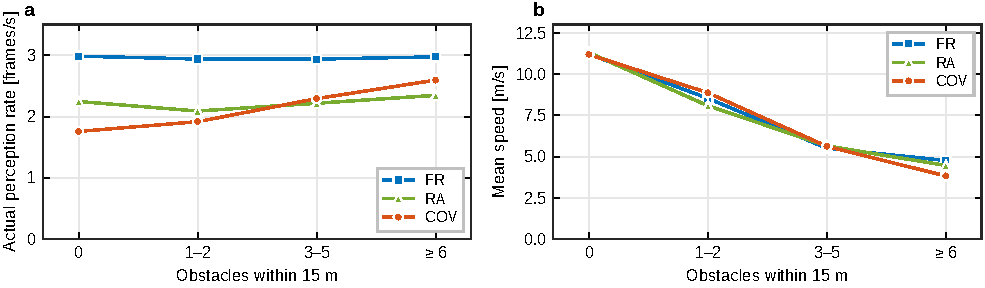
\includegraphics[width=\textwidth]{Fig5.pdf}
\caption{Frame rate (\textbf{a}) and mean speed (\textbf{b}) versus the number of obstacles within a radius of 15~m
(SN, $v_{\mathrm{des}} = 15$~m/s, $\fmax = 3$~Hz; total flight time over 60 worlds)}
\label{fig:dens}
\end{figure}

\subsection{Claim 4: the geometric criterion outperforms the remaining safe time}\label{sec:r4}

\runin{Prediction.} RA and COV use almost the same number of inferences at the same cap (ratio 0.93--0.98 at 3~Hz), so
comparing them separates the role of the \emph{timing} of the captures from that of their \emph{number}. The remaining
safe time of RA is computed with respect to the objects already in the memory and to a hypothetical object at the
boundary of the trusted range along the flight direction; it does not consider the actual path and the occluded space
along it. If the thesis holds, COV should have a lower collision rate at the same number of frames, in particular when
the path departs from the current flight direction.

\runin{Result.} Pooling 1.5--5~Hz, the collision rate of COV is lower than that of RA in SN (2.4\,\% and 3.9\,\%,
$p = 0.033$) and SH (8.2\,\% and 12.2\,\%, $p = 0.015$); in SE, it is 0.3\,\% and 1.1\,\% ($p = 0.11$).
Figure~\ref{fig:dens}a shows that the two schedulers allocate frames differently: RA captures more than COV with no
object nearby (2.24 and 1.76~frames/s) and less in dense regions (2.35 and 2.59~frames/s). This difference is
consistent with the mechanism of condition~\eqref{eq:cov}: when the path turns away from the current flight direction
to go around an object, it enters the unobserved space behind the object (Fig.~\ref{fig:cov}b) and the coverage
condition triggers a frame, whereas the remaining safe time with respect to known objects does not depend on the path.
The same situation is decisive in the flight experiments of RAPTOR: an obstacle placed behind a corner was avoided only
by the planner that enforced visibility of the unknown region and turned the camera toward it, while the other three
planners collided~\cite{zhou2021}.

\runin{Conclusion.} The results support placing the trigger criterion on the planned path and the observed space
rather than on the distance to known objects.

\subsection{Claim 5: the camera field of view is a prerequisite}\label{sec:r5}

\runin{Prediction.} The coverage condition saves inferences only if each frame observes a sufficiently wide part of the
space that the path will use, including when the path turns to go around an object. The horizontal field of view
should therefore matter more than the detection range, and the advantage of COV should depend on the camera.

\runin{Result.} Table~\ref{tab:camera} and Fig.~\ref{fig:cam} compare four configurations. The two narrow cameras
($62^\circ$ and $66^\circ$) have a longer trusted range (30~m versus 26~m), but collision rates 4.9--5.4 times higher
in SN (10.7\,\% and 11.9\,\% versus 2.2\,\%) and 3.9--4.6 times higher in SH, rates of stuck runs 6--11 times higher,
and times to goal 15\,\% (SN) to 42\,\% (SH) longer. Raising the cap does not compensate for a narrow field of view:
at 5~Hz, the collision rate of these two cameras in SN is still 6.4--7.2\,\%, higher than that of the wide camera at
1.5~Hz (3.3\,\%). In SE, almost all collisions of the narrow cameras occur in the two scene types with objects close to
both sides of the route (avenue, street canyon). The $640\times360$ network on the wide camera costs 4 times as much
computation per inference and has a latency of 320~ms, so its actual frame rate is limited to about 2.9~frames/s and
its collision rate is higher than that of the $320\times180$ network (SN 3.1\,\% and 2.2\,\%, $p = 0.041$; SH
10.9\,\% and 7.0\,\%, $p = 0.0003$). With the narrow cameras or the $640\times360$ network, COV has a higher collision
rate than FR in some cells (v2 in SN: 12.8\,\% and 8.7\,\%, $p = 0.0005$; Module~3 in SH: 36.1\,\% and 28.3\,\%,
$p = 0.002$; $640\times360$ network: SN $p = 0.024$, SH $p = 0.001$).

\runin{Conclusion.} The results are consistent with the mechanism of the coverage condition: when the free space that
each frame observes is smaller (narrow field of view) or is updated more slowly (large latency), skipping frames on
the basis of that space leaves little room. The inference savings of COV come with equivalent safety only with a
wide-angle camera and a low-latency network. This is also consistent with earlier analyses showing that a limited
field of view forces the motion to be restricted to the visible region~\cite{misyats2025}.

\begin{table}[t]
\caption{Camera configurations and static collision rates (COV and FR pooled, $\fmax = 1.5$--5~Hz)}\label{tab:camera}
\renewcommand{\thefootnote}{\alph{footnote}}% table notes: lower-case letters
\setlength{\tabcolsep}{3.6pt}
\begin{tabular}{@{}lcccccccc@{}}
\toprule
Camera\footnotemark[1] & Field of & Network & Inference & $\Reff$ & $v_{\max}$\footnotemark[2] &
\multicolumn{3}{c}{Static collisions [\%]} \\
\cmidrule(l){7-9}
 & view & input & [ms] & [m] & [m/s] & SN & SH & SE \\
\midrule
Module 3 Wide\footnotemark[3] & $102^\circ\times70^\circ$ & $320\times180$ & 80 & 26 & 15 & 2.2 & 7.0 & 0.3 \\
Module 3 Wide & $102^\circ\times70^\circ$ & $640\times360$ & 320 & 30 & 15 & 3.1 & 10.9 & 1.0 \\
Camera Module v2 & $62^\circ\times49^\circ$ & $280\times210$ & 82 & 30 & 13.1 & 10.7 & 27.6 & 6.3 \\
Camera Module 3 & $66^\circ\times40^\circ$ & $320\times180$ & 80 & 30 & 10.7 & 11.9 & 32.2 & 7.4 \\
\botrule
\end{tabular}
\footnotetext[1]{Raspberry Pi; horizontal field of view from the manufacturer's documentation (Module 3, Module 3
Wide~\cite{rpi_cm3}; Camera Module v2~\cite{rpi_doc}), vertical field of view computed for the image fed to the
network. Each cell contains 2\,880 runs (SN) or 1\,440 runs (SH, SE).}
\footnotetext[2]{Maximum speed at which the path ahead remains in the image when the UAV pitches forward.}
\footnotetext[3]{Default configuration.}
\end{table}

\begin{figure}[t]
\centering
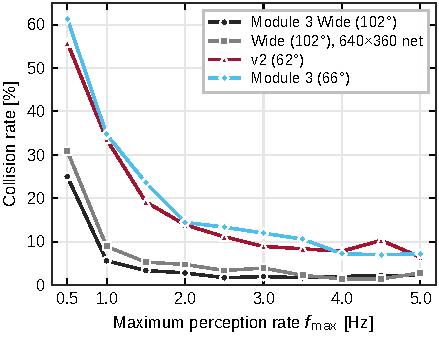
\includegraphics[width=0.5\textwidth]{Fig6.pdf}
\caption{Collision rate with static objects versus the rate cap for the four camera configurations (SN, COV and FR
pooled, 360 runs per point)}
\label{fig:cam}
\end{figure}

% =====================================================================================================================
\section{Discussion}\label{sec:discussion}

\subsection{Implications and relation to prior work}

The benefit of removing 28--50\,\% of the inferences should be understood in terms of accelerator resources rather
than flight energy: on the micro aerial vehicle studied in~\cite{boroujerdian2021}, computation accounts for less than
0.05\,\% of the total energy. The freed computation can serve tasks that share the CPU or GPU~\cite{wofk2019}, a larger
network at the same mean rate, or a reserve for dense stretches. Compared with Zhuyi and D3~\cite{hsiao2022,gog2022},
the coverage condition derives the perception need not from the detected objects but from the unobserved space along
the path, and thus directly addresses the occluded space that~\cite{hsiao2022} leaves open; RoboRun sets its decision
deadline from visibility and stopping distance and adapts the decision rate to the heterogeneity of
space~\cite{boroujerdian2021}, without relying on the unobserved space along the path. Compared with planners that
keep a stopping trajectory in known free space~\cite{liu2016,tordesillas2021}, it uses the same reasoning to decide
when to measure. Compared with RAPTOR~\cite{zhou2021}, which adapts the trajectory and the yaw angle so that the point
where the path leaves known free space is observed early enough to stop, the coverage condition leaves the motion to the
planner and decides when to run the inference. Compared with NanoMap~\cite{florence2018}, the free-space test is the same, but here it decides the
timing of inference. The saturation of the collision rate from about 2~Hz agrees with the observations in automated
driving that the required processing rate is finite and scenario-dependent~\cite{zhao2021,hsiao2022}.

\subsection{Scope and limitations}

\begin{itemize}
\item \emph{Simulation.} The depth network is replaced by a synthetic error model on ray-cast depth images (no colour
rendering, no ground plane), and the camera parameters are taken from published specifications. The results need to
be verified on hardware, where many related works have flown~\cite{loquercio2021,simon2023,tordesillas2021,pant2021}.
\item \emph{Guarantees.} Proposition~\ref{prop:cov} is a local condition for the scheduling decision, under the
assumptions that the observed free space is correct and that the speed does not increase within $\tauh$;
\eqref{eq:need} contains no acceleration term. The closed loop has no formal certificate (Remark~\ref{rem:scope}): the
CBF filter is discrete at 100~Hz, so safety between steps is not formally guaranteed~\cite{breeden2022,bahati2024};
the filter uses a slack variable~\cite{yaghoubi2021}; the inflated radius jumps at each Kalman update; and the MPC with
a terminal stop constraint and CBF rows over the first steps has no proof of recursive feasibility~\cite{zeng2021}.
\item \emph{Static objects.} The crossing vehicles in SH are updated only frame by frame; the 56 collisions with them
at caps from 1.5~Hz are outside the scope.
\item \emph{Remaining collisions.} From 2~Hz, the collision rate pooled over the four schedulers is 2.4--3.2\,\% in SN
and 8.3\,\% in SH and does not decrease with the cap (Section~\ref{sec:r1}); this floor is not due to the perception
rate, and the analysis of its origin is outside the scope of this paper.
\item \emph{Continuously dense scenes.} In SH, COV has a collision rate of 8.2\,\% versus 5.8\,\% for FR
($p = 0.098$); the data do not allow equivalence to be claimed for this type of scene.
\item \emph{Representation.} Vertical cylinders are conservative for horizontally elongated objects seen at an angle;
the vertical direction is taken from the true attitude at the capture time; the range $\Reff$ was measured before the
transition to the cylinder model.
\end{itemize}

% =====================================================================================================================
\section{Conclusion}\label{sec:conclusion}

This paper asked when a low-cost quadrotor needs to run a delayed monocular depth network, and answered with a
geometric condition: when the planned path, up to the distance needed to stop after the next result, is no longer
contained in the observed free space. This condition is sufficient for skipping an inference not to remove the ability
to stop within observed space. Combined with a hard rate cap and a perception-range speed limit, it leads to
consequences verified in 36\,000 simulated runs: at the same cap, the number of inferences decreases by 28--50\,\% in
the nominal and everyday scenarios without a significant difference in safety; the frame rate increases with obstacle
density; at the same number of inferences, the geometric criterion yields a lower collision rate than the
remaining-safe-time criterion; and at the same low budget, the number of failed runs decreases. The condition for
these results to hold is a wide-angle camera with a low-latency network. The next steps are to include an acceleration
term in the coverage condition and to verify the approach on hardware.

% =====================================================================================================================
\backmatter

\section*{Statements and Declarations}

\bmhead{Funding}
No funding was received for conducting this study.

\bmhead{Competing interests}
The author has no competing interests to declare that are relevant to the content of this article.

\bmhead{Ethics approval and consent}
Not applicable: the study is a simulation study without human or animal participants.

\bmhead{Data availability}
The per-run results of the 36\,000 simulated flights and the scripts that produce the tables and figures are
available in the GitHub repository \url{https://github.com/nxbnxb1/project1}.

\bmhead{Code availability}
The MATLAB/Simulink source code and the GitHub Actions workflows used to run the experiments are available in the
same repository, \url{https://github.com/nxbnxb1/project1}.

\bmhead{Author contributions}
[withheld in the public copy]

\begin{thebibliography}{99}
% BEGIN AUTO REFS (generated by docs/paper/build_refs.py --inline from docs/paper/references.py; do not edit)
\bibitem{falanga2019} Falanga, D., Kim, S., Scaramuzza, D.: How fast is too fast? The role of perception latency in high-speed sense and avoid. IEEE Robot. Autom. Lett. \textbf{4}(2), 1884--1891 (2019). \url{https://doi.org/10.1109/LRA.2019.2898117}

\bibitem{loquercio2021} Loquercio, A., Kaufmann, E., Ranftl, R., M\"uller, M., Koltun, V., Scaramuzza, D.: Learning high-speed flight in the wild. Sci. Robot. \textbf{6}(59), eabg5810 (2021). \url{https://doi.org/10.1126/scirobotics.abg5810}

\bibitem{yang2024b} Yang, L., Kang, B., Huang, Z., Zhao, Z., Xu, X., Feng, J., Zhao, H.: Depth Anything V2. In: Adv. Neural Inf. Process. Syst. (NeurIPS) \textbf{37}, 21875--21911 (2024). \url{https://doi.org/10.52202/079017-0688}

\bibitem{wofk2019} Wofk, D., Ma, F., Yang, T.-J., Karaman, S., Sze, V.: FastDepth: Fast monocular depth estimation on embedded systems. In: Proc. Int. Conf. Robot. Autom. (ICRA), pp. 6101--6108 (2019). \url{https://doi.org/10.1109/ICRA.2019.8794182}

\bibitem{simon2023} Simon, N., Majumdar, A.: MonoNav: MAV navigation via monocular depth estimation and reconstruction. In: Ang Jr, M.H., Khatib, O. (eds.) Experimental Robotics (ISER 2023). Springer Proc. Adv. Robot., pp. 415--426. Springer, Cham (2024). \url{https://doi.org/10.1007/978-3-031-63596-0_37}

\bibitem{liu2016} Liu, S., Watterson, M., Tang, S., Kumar, V.: High speed navigation for quadrotors with limited onboard sensing. In: Proc. IEEE Int. Conf. Robot. Autom. (ICRA), pp. 1484--1491 (2016). \url{https://doi.org/10.1109/ICRA.2016.7487284}

\bibitem{zhao2021} Zhao, H., Hari, S.K.S., Tsai, T., Sullivan, M.B., Keckler, S.W., Zhao, J.: Suraksha: A framework to analyze the safety implications of perception design choices in AVs. In: Proc. IEEE 32nd Int. Symp. Softw. Reliab. Eng. (ISSRE), pp. 434--445 (2021). \url{https://doi.org/10.1109/ISSRE52982.2021.00052}

\bibitem{hsiao2022} Hsiao, Y.-S., Hari, S.K.S., Filipiuk, M., Tsai, T., Sullivan, M.B., Reddi, V.J., Singh, V., Keckler, S.W.: Zhuyi: Perception processing rate estimation for safety in autonomous vehicles. In: Proc. 59th ACM/IEEE Design Autom. Conf. (DAC), pp. 289--294 (2022). \url{https://doi.org/10.1145/3489517.3530445}

\bibitem{gog2022} Gog, I., Kalra, S., Schafhalter, P., Gonzalez, J.E., Stoica, I.: D3: A dynamic deadline-driven approach for building autonomous vehicles. In: Proc. 17th Eur. Conf. Comput. Syst. (EuroSys), pp. 453--471 (2022). \url{https://doi.org/10.1145/3492321.3519576}

\bibitem{boroujerdian2021} Boroujerdian, B., Ghosal, R., Cruz, J., Plancher, B., Reddi, V.J.: RoboRun: A robot runtime to exploit spatial heterogeneity. In: Proc. 58th ACM/IEEE Design Autom. Conf. (DAC), pp. 829--834 (2021). \url{https://doi.org/10.1109/DAC18074.2021.9586280}

\bibitem{pant2021} Pant, Y.V., Abbas, H., Mohta, K., Quaye, R.A., Nghiem, T.X., Devietti, J., Mangharam, R.: Anytime computation and control for autonomous systems. IEEE Trans. Control Syst. Technol. \textbf{29}(2), 768--779 (2021). \url{https://doi.org/10.1109/TCST.2020.2979388}

\bibitem{tordesillas2021} Tordesillas, J., Lopez, B.T., Everett, M., How, J.P.: FASTER: Fast and safe trajectory planner for navigation in unknown environments. IEEE Trans. Robot. \textbf{38}(2), 922--938 (2022). \url{https://doi.org/10.1109/TRO.2021.3100142}

\bibitem{zhou2021} Zhou, B., Pan, J., Gao, F., Shen, S.: RAPTOR: Robust and perception-aware trajectory replanning for quadrotor fast flight. IEEE Trans. Robot. \textbf{37}(6), 1992--2009 (2021). \url{https://doi.org/10.1109/TRO.2021.3071527}

\bibitem{florence2018} Florence, P.R., Carter, J., Ware, J., Tedrake, R.: NanoMap: Fast, uncertainty-aware proximity queries with lazy search over local 3D data. In: Proc. IEEE Int. Conf. Robot. Autom. (ICRA), pp. 7631--7638 (2018). \url{https://doi.org/10.1109/ICRA.2018.8463195}

\bibitem{aldana2023} Aldana-L\'opez, R., Arag\"u\'es, R., Sag\"u\'es, C.: Latency vs precision: Stability preserving perception scheduling. Automatica \textbf{155}, 111123 (2023). \url{https://doi.org/10.1016/j.automatica.2023.111123}

\bibitem{huang2020} Huang, C., Xu, S., Wang, Z., Lan, S., Li, W., Zhu, Q.: Opportunistic intermittent control with safety guarantees for autonomous systems. In: Proc. 57th ACM/IEEE Design Autom. Conf. (DAC), pp. 1--6 (2020). \url{https://doi.org/10.1109/DAC18072.2020.9218742}

\bibitem{zhou2019} Zhou, B., Gao, F., Wang, L., Liu, C., Shen, S.: Robust and efficient quadrotor trajectory generation for fast autonomous flight. IEEE Robot. Autom. Lett. \textbf{4}(4), 3529--3536 (2019). \url{https://doi.org/10.1109/LRA.2019.2927938}

\bibitem{lin2020} Lin, J., Zhu, H., Alonso-Mora, J.: Robust vision-based obstacle avoidance for micro aerial vehicles in dynamic environments. In: Proc. IEEE Int. Conf. Robot. Autom. (ICRA), pp. 2682--2688 (2020). \url{https://doi.org/10.1109/ICRA40945.2020.9197481}

\bibitem{falanga2018} Falanga, D., Foehn, P., Lu, P., Scaramuzza, D.: PAMPC: Perception-aware model predictive control for quadrotors. In: Proc. IEEE/RSJ Int. Conf. Intell. Robots Syst. (IROS), pp. 1--8 (2018). \url{https://doi.org/10.1109/IROS.2018.8593739}

\bibitem{misyats2025} Misyats, M., Harms, M., Nissov, M., Jacquet, M., Alexis, K.: Embedded safe reactive navigation for multirotors systems using control barrier functions. In: Proc. Int. Conf. Unmanned Aircr. Syst. (ICUAS), pp. 697--704 (2025). \url{https://doi.org/10.1109/ICUAS65942.2025.11007827}

\bibitem{ames2017} Ames, A.D., Xu, X., Grizzle, J.W., Tabuada, P.: Control barrier function based quadratic programs for safety critical systems. IEEE Trans. Autom. Control \textbf{62}(8), 3861--3876 (2017). \url{https://doi.org/10.1109/TAC.2016.2638961}

\bibitem{ames2019} Ames, A.D., Coogan, S., Egerstedt, M., Notomista, G., Sreenath, K., Tabuada, P.: Control barrier functions: Theory and applications. In: Proc. 18th Eur. Control Conf. (ECC), pp. 3420--3431 (2019). \url{https://doi.org/10.23919/ECC.2019.8796030}

\bibitem{wang2017} Wang, L., Ames, A.D., Egerstedt, M.: Safety barrier certificates for collisions-free multirobot systems. IEEE Trans. Robot. \textbf{33}(3), 661--674 (2017). \url{https://doi.org/10.1109/TRO.2017.2659727}

\bibitem{xiao2019} Xiao, W., Belta, C.: Control barrier functions for systems with high relative degree. In: Proc. IEEE 58th Conf. Decis. Control (CDC), pp. 474--479 (2019). \url{https://doi.org/10.1109/CDC40024.2019.9029455}

\bibitem{zeng2021} Zeng, J., Zhang, B., Sreenath, K.: Safety-critical model predictive control with discrete-time control barrier function. In: Proc. Am. Control Conf. (ACC), pp. 3882--3889 (2021). \url{https://doi.org/10.23919/ACC50511.2021.9483029}

\bibitem{rosolia2020} Rosolia, U., Ames, A.D.: Multi-rate control design leveraging control barrier functions and model predictive control policies. IEEE Control Syst. Lett. \textbf{5}(3), 1007--1012 (2021). \url{https://doi.org/10.1109/LCSYS.2020.3008326}

\bibitem{breeden2022} Breeden, J., Garg, K., Panagou, D.: Control barrier functions in sampled-data systems. IEEE Control Syst. Lett. \textbf{6}, 367--372 (2022). \url{https://doi.org/10.1109/LCSYS.2021.3076127}

\bibitem{bahati2024} Bahati, G., Ong, P., Ames, A.D.: Sample-and-hold safety with control barrier functions. In: Proc. Am. Control Conf. (ACC), pp. 5169--5176 (2024). \url{https://doi.org/10.23919/ACC60939.2024.10645060}

\bibitem{molnar2022} Molnar, T.G., Kiss, A.K., Ames, A.D., Orosz, G.: Safety-critical control with input delay in dynamic environment. IEEE Trans. Control Syst. Technol. \textbf{31}(4), 1507--1520 (2023). \url{https://doi.org/10.1109/TCST.2022.3227451}

\bibitem{taylor2020} Taylor, A.J., Ong, P., Cort\'es, J., Ames, A.D.: Safety-critical event triggered control via input-to-state safe barrier functions. IEEE Control Syst. Lett. \textbf{5}(3), 749--754 (2021). \url{https://doi.org/10.1109/LCSYS.2020.3005101}

\bibitem{yang2019} Yang, G., Belta, C., Tron, R.: Self-triggered control for safety critical systems using control barrier functions. In: Proc. Am. Control Conf. (ACC), pp. 4454--4459 (2019). \url{https://doi.org/10.23919/ACC.2019.8814657}

\bibitem{dean2021} Dean, S., Taylor, A.J., Cosner, R.K., Recht, B., Ames, A.D.: Guaranteeing safety of learned perception modules via measurement-robust control barrier functions. In: Proc. 2020 Conf. Robot Learning (CoRL), PMLR \textbf{155}, 654--670 (2021)

\bibitem{yang2023} Yang, S., Pappas, G.J., Mangharam, R., Lindemann, L.: Safe perception-based control under stochastic sensor uncertainty using conformal prediction. In: Proc. 62nd IEEE Conf. Decis. Control (CDC), pp. 6072--6078 (2023). \url{https://doi.org/10.1109/CDC49753.2023.10384075}

\bibitem{yaghoubi2021} Yaghoubi, S., Fainekos, G., Yamaguchi, T., Prokhorov, D., Hoxha, B.: Risk-bounded control with Kalman filtering and stochastic barrier functions. In: Proc. 60th IEEE Conf. Decis. Control (CDC), pp. 5213--5219 (2021). \url{https://doi.org/10.1109/CDC45484.2021.9683756}

\bibitem{zhu2019} Zhu, H., Alonso-Mora, J.: Chance-constrained collision avoidance for MAVs in dynamic environments. IEEE Robot. Autom. Lett. \textbf{4}(2), 776--783 (2019). \url{https://doi.org/10.1109/LRA.2019.2893494}

\bibitem{laine2020} Laine, F., Chiu, C.-Y., Tomlin, C.: Eyes-closed safety kernels: Safety of autonomous systems under loss of observability. In: Robotics: Science and Systems XVI (2020). \url{https://doi.org/10.15607/RSS.2020.XVI.096}

\bibitem{barshalom2002} Bar-Shalom, Y.: Update with out-of-sequence measurements in tracking: Exact solution. IEEE Trans. Aerosp. Electron. Syst. \textbf{38}(3), 769--777 (2002). \url{https://doi.org/10.1109/TAES.2002.1039398}

\bibitem{garcia2021} Garc\'ia-Fern\'andez, \'A.F., Yi, W.: Continuous-discrete multiple target tracking with out-of-sequence measurements. IEEE Trans. Signal Process. \textbf{69}, 4699--4709 (2021). \url{https://doi.org/10.1109/TSP.2021.3100999}

\bibitem{rpi_cm3} Raspberry Pi Ltd: Raspberry Pi Camera Module 3 (Standard, NoIR, Wide, NoIR Wide), product brief (2024). \url{https://datasheets.raspberrypi.com/camera/camera-module-3-product-brief.pdf}. Accessed 18 October 2026

\bibitem{ranftl2020} Ranftl, R., Lasinger, K., Hafner, D., Schindler, K., Koltun, V.: Towards robust monocular depth estimation: Mixing datasets for zero-shot cross-dataset transfer. IEEE Trans. Pattern Anal. Mach. Intell. \textbf{44}(3), 1623--1637 (2022). \url{https://doi.org/10.1109/TPAMI.2020.3019967}

\bibitem{yang2024a} Yang, L., Kang, B., Huang, Z., Xu, X., Feng, J., Zhao, H.: Depth Anything: Unleashing the power of large-scale unlabeled data. In: Proc. IEEE/CVF Conf. Comput. Vis. Pattern Recognit. (CVPR), pp. 10371--10381 (2024). \url{https://doi.org/10.1109/CVPR52733.2024.00987}

\bibitem{bhattacharya2024} Bhattacharya, A., Cannici, M., Rao, N., Tao, Y., Kumar, V., Matni, N., Scaramuzza, D.: Monocular event-based vision for obstacle avoidance with a quadrotor. In: Proc. 8th Conf. Robot Learning (CoRL), PMLR \textbf{270}, 4826--4843 (2025)

\bibitem{mehrotra1992} Mehrotra, S.: On the implementation of a primal--dual interior point method. SIAM J. Optim. \textbf{2}(4), 575--601 (1992). \url{https://doi.org/10.1137/0802028}

\bibitem{lee2010} Lee, T., Leok, M., McClamroch, N.H.: Geometric tracking control of a quadrotor UAV on SE(3). In: Proc. 49th IEEE Conf. Decis. Control (CDC), pp. 5420--5425 (2010). \url{https://doi.org/10.1109/CDC.2010.5717652}

\bibitem{rpi_doc} Raspberry Pi Ltd: Camera (Raspberry Pi documentation, hardware specifications). \url{https://www.raspberrypi.com/documentation/accessories/camera.html} (2026). Accessed 18 October 2026

% END AUTO REFS
\end{thebibliography}

\section*{Author biography}
[withheld in the public copy]

\end{document}
